\newpage
\section{Visualization}
Visualization is a key component of data analysis since it can provide insights on its own. It relies on the fact that a human can easily recognize patterns. Usually they are 2D with color.
\subsection{Classical}
There are basically four categories of classical visualization, depending on the type of data:
\begin{itemize}
	\item \textbf{Array plot}
	\item \textbf{Scatter plot}
	\item \textbf{Histograms}
	\item \textbf{Graphs}
\end{itemize}

\subsubsection{Array plot}
Usually a two dimensional space organized as a \textbf{grid}. Each row represents an instance and the columns represent numerical features. Each element in the array is then \textbf{colored} according to the feature value of the given instance and a color map. Usually there is also a color scale.

\begin{example}[Game of Thrones]
	In this example we see the adjacency matrix for the relationship between all the characters in Game of Thrones.
	\begin{center}
		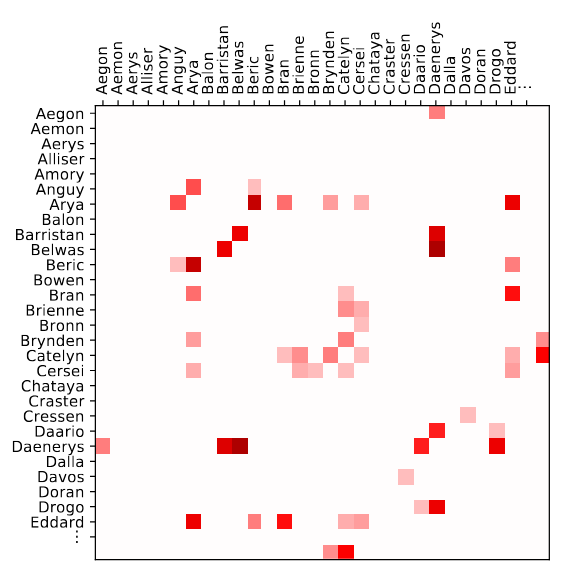
\includegraphics[scale=0.4]{got.png}
	\end{center}
\end{example}

The strengths of this type of visualization are that a lot of \textbf{qualitative information} can be gathered and it's really helpful for spotting \textbf{missing values} or \textbf{lack of normalization} before a more advanced data analysis.\\
At the same time, it gets quickly \textbf{overwhelming} with large datasets and it's \textbf{not very precise} about the values and their distribution.
\newpage
\subsubsection{Histograms}
This type of visualization focuses on just one feature so that more information can be extracted. The values are indicated by the position on the $x$-axis while the number of instances for each feature by the position on the $y$-axis.

\begin{example}[UCI Wholesale]
	In this example we have one Histogram for each product. Since there are different levels of spending, the result shows mainly the large spenders. To avoid this we apply the following \textbf{preprocessing}:
	\begin{equation*}
		z = \log(1+x)
	\end{equation*}
	and \textbf{standardization} (subtract the mean and divide by standard deviation).
	\begin{center}
		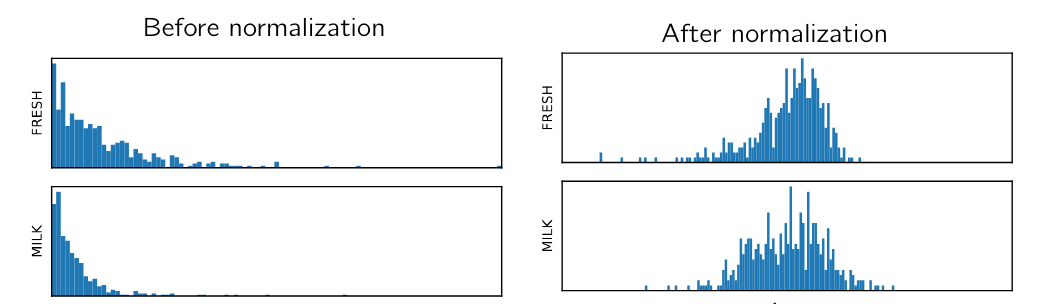
\includegraphics[scale=0.3]{histogram.png}
	\end{center}
\end{example}

Histograms are very \textbf{precise} in characterizing the distribution of individual features but they do not highlight correlations between them. Also, not practical with a high-dimensional dataset since we would need an Histogram for every feature.

\subsubsection{Scatter plots}
Scatter plots consider two features (on the axis) at the same time to find correlations. To improve them we can use \textbf{transparency} and build a black \textbf{outline} to better find outliers.

\begin{example}
	A scatter plot with the same dataset of the last example:
	\begin{center}
		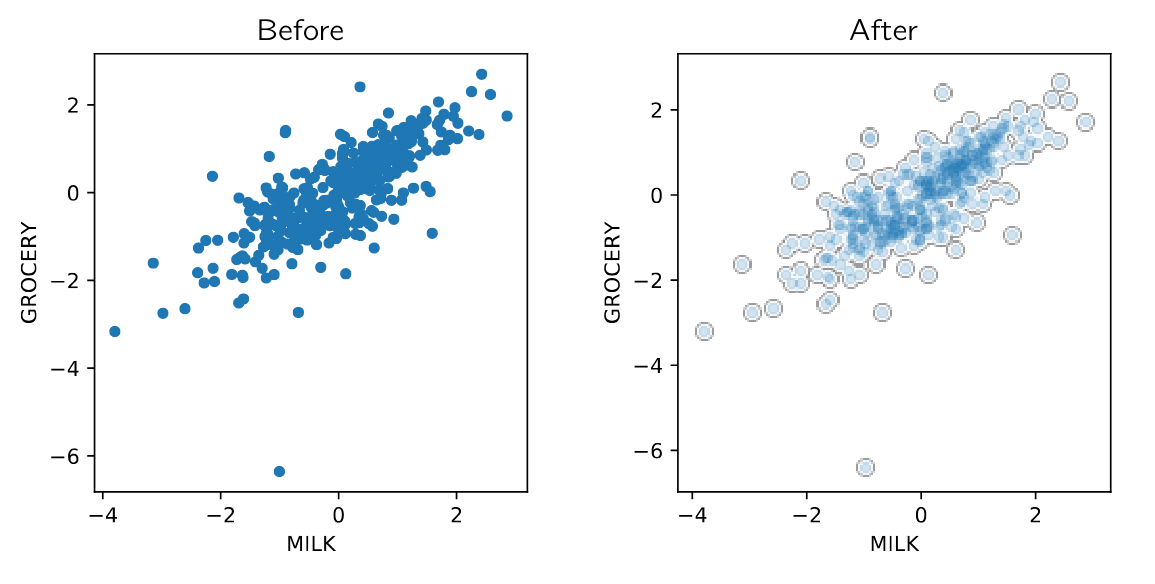
\includegraphics[scale=0.3]{scatter.png}
	\end{center}
\end{example}

\subsubsection{Graph visualization}
To visualize a graph, we arrange the nodes in a two-dimensional layout (e.g. a ring) and we draw lines between the nodes connected by an edge. If the edge strength is a real value, draw the line only if above a certain threshold.\\
It works well with a \textbf{sparse} graph.

\newpage
\begin{example}
	A \textbf{chord plot}, where the line used for each pair of nodes $(x_i, x_j)$ is the following parameterized curve
	\begin{equation}
		x(t) = x_i\cdot p^t + x_j\cdot (1-t)^p
	\end{equation}
	which is a line when $p=1$, otherwise it's a curve attracted to the center, making connections between nearby nodes more visible.
	\begin{center}
		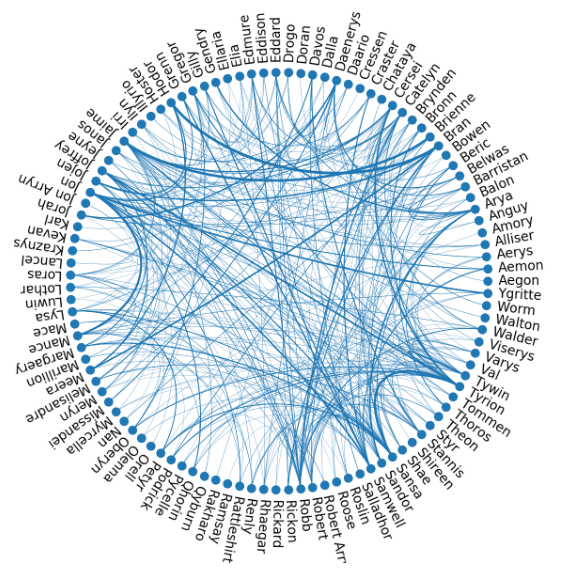
\includegraphics[scale=0.3]{chordplot}
	\end{center}
\end{example}

\subsection{Low dimensional embedding}
Low-dimensional embedding aims to construct a \textit{scatter plot} where the axes do not carry specific meaning but it's the \textbf{distance} that represent distances and similarities in the original input space.

\paragraph{Gradient descent}
Assuming you want to find the minimum of a function $J(\theta)$, follow:
\begin{enumerate}
	\item Initialize $\theta$ with a random value
	\item Apply repeatedly 
	\begin{equation}
		\theta \longleftarrow \theta - \gamma \bigtriangledown_\theta J(\theta)
	\end{equation}
	Where $\gamma$ is the \textbf{learning rate} set  appropriately to avoid slowing down the convergence or create instability.
	\item Return $\theta$
\end{enumerate}
\begin{note}
	\textbf{Initialization} is important to reach a good minimum. Gradient descent can be made to converge quickly by following the direction of the \textbf{average} of past gradients.
\end{note}

\subparagraph{Chain rule} Suppose that a \textbf{parameter of interest} $\theta_q$ (one element of the vector) is linked to $z$ through a mapping
\begin{equation*}
	\theta_q \longrightarrow a \longrightarrow b \longrightarrow z
\end{equation*}
then the derivative of the parameter of interest is the product of the local derivatives along the path
\begin{equation*}
	\frac{\delta z}{\delta \theta_q} = \frac{\delta z}{\delta b} \cdot \frac{\delta b}{\delta a} \cdot \frac{\delta a}{\delta \theta_q}
\end{equation*}
In practice the parameter of interest could be linked to the output through multiple paths. The rule is therefore extended by enumerating all the paths:
\begin{equation*}
	\frac{\delta z}{\delta \theta_q} = \sum_i \sum_j \frac{\delta z}{\delta b_j} \cdot \frac{\delta b_j}{\delta a_i} \cdot \frac{\delta a_i}{\delta \theta_q}
\end{equation*}

\subsubsection{MDS}
Multi Dimensional Scaling (MDS) is a low-dimensional embedding technique that generates for each instance a \textbf{vector} in low dimensions. These vectors are optimized so that the distances between points in low-dimensional space replicate the true distances between corresponding instances.\\
It follows this notation:
\begin{itemize}
	\item $d_{ij}$: \textbf{true distance} between the two instances, usually the Euclidean distance in the input space
	\begin{equation*}
		d_{ij} = \lvert\lvert x_i - x_j \rvert\rvert
	\end{equation*}
	\item $y_i$:  representation of the \textbf{instance} in low dimensional space (usually two dimensions)
	\item $\hat{d}_{ij}$: \textbf{distance} between the two instances in the low-dimensional space
	\begin{equation*}
		\hat{d}_{ij} = \lvert\lvert y_i - y_j \rvert\rvert
	\end{equation*}
\end{itemize}

\paragraph{Metric MDS}
It finds the embedding that minimizes the discrepancy between $d_{ij}$ and $\hat{d}_{ij}$ by minimizing
\begin{equation}
	\text{stress}(y_1, \ldots, y_N) = \bigg(\frac{\sum_{i<j}(d_{ij} - \hat{d}_{ij})^2}{\sum_{i<j}d^2_{ij}}\bigg)^\frac{1}{2}
\end{equation} 
The idea is similar to connecting the data points with strings, each one with a specific length in a relaxed state, which is determined by the input space. The Metric MDS solution is given by the relaxed state of the spring system.

\begin{center}
	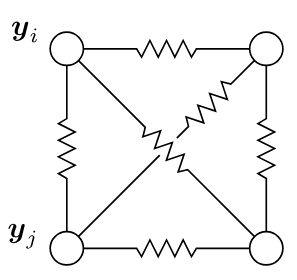
\includegraphics[scale=0.3]{mds}
\end{center}

The algorithm starts with a random initialization of the points $y_1, \ldots, y_N$ and iteratively updates them to minimize the \textit{stress} function. The optimization procedure is usually done multiple times with different seeds.\\
Another technique is with the \textbf{gradient descent}, considering a slightly different stress function
\begin{equation}
	\text{stress}(y) = C \cdot \big(\sum_{i<j} ( \Delta_{ij} - d_{ij})^2\big)^\frac{1}{2} \qquad\qquad \Delta_{ij} = \lvert\lvert y_i - y_j \rvert\rvert 
\end{equation}
and with the gradient given by
\begin{equation}
	\frac{\delta_{\text{stress}}}{\delta_{y_k}} = C \cdot \sum_{i<j} \frac{\Delta_{ij}}{\lvert\lvert \Delta \rvert\rvert} \cdot \frac{y_i - y_y}{\lvert\lvert y_i - y_j \rvert\rvert} \cdot (\delta_{ik} - \delta_{jk}) \qquad\qquad \Delta = (\Delta_{ij})_{i<j}
\end{equation}

\paragraph{Non Metric MDS}
Extends Metric MDS with the application of a fine transformation $f$ (learnt from data) to the distances. This allows for handling mismatches, enabling points that are relatively close in space to be very close in embedded space and points that are relatively far in space to be very far in embedded space.
\begin{equation}
	\text{stress}(y_1, \ldots, y_N) = \bigg(\frac{\sum_{i<j}(d_{ij} - f(\hat{d}_{ij}))^2}{\sum_{i<j}d^2_{ij}}\bigg)^\frac{1}{2}
\end{equation} 
\newpage
\paragraph{Comparison} Non Metric MDS matches more faithfully true distances between data points (up to an affine transformation) and appears crowded near the center of the visualization.
\begin{figure}[!h]
	\hfill
	\subfigure[Metric MDS]{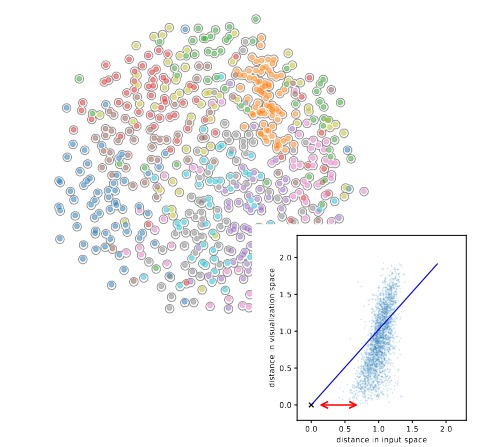
\includegraphics[scale=0.4]{mmds}}
	\hfill
	\subfigure[Non Metric MDS]{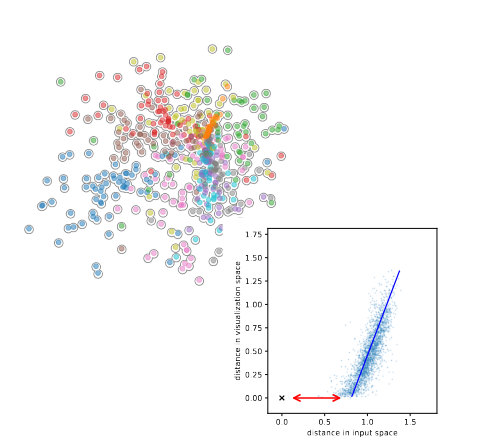
\includegraphics[scale=0.4]{nmds}}
	\hfill
\end{figure}

\subsubsection{T-SNE}
This method ensures to preserve \textbf{similarities}, promoting a correct representation of small distances and tolerating large errors for large distances.\\
It aims to learn embedding coordinates such that similarities between points matches similarities in embedded space. The collection of pairwise \textbf{similarities} are viewed as two probabilities distribution defined over the pair of points: $p$ in the \textit{input space} and $q$ in the \textit{embedded space}.\\
The embedding $\mathbf{y} = (\mathbf{y}_1, \ldots, \mathbf{y}_N)$ is such that minimizes the KL divergence
\begin{equation}
	D_{KL}(p \vert\vert q(\mathbf{y})) = \sum_{ij} p_{ij} \log\frac{p_{ij}}{q_{ij}(\mathbf{y})}
\end{equation}
This function is minimized through \textbf{gradient descent}:
\begin{equation*}
	\mathbf{y} \longleftarrow y - \gamma \cdot \bigtriangledown D_{KL}(p \vert\vert q(\mathbf{y}))
\end{equation*}

\paragraph{Modeling} Similarities are modeled using different functions for the input and the embedded space because of the \textbf{concentration of distances}.

\begin{definition}[Concentration of distances]
	The squared Euclidean distance between two points is given as a sum over individual dimensions:
	\begin{equation}
		\lvert\lvert \mathbf{x} - \mathbf{x}' \rvert\rvert ^ 2 = \sum_{t=1}^{d} (x_t - x_t')^2
	\end{equation}
	Assuming dimensions-wise squared distances are iid. (e.g. random data), the expected square distance grows linearly with $d$ but the standard deviation grows with $\sqrt{d}$ (cf. law of large numbers).
	\begin{center}
		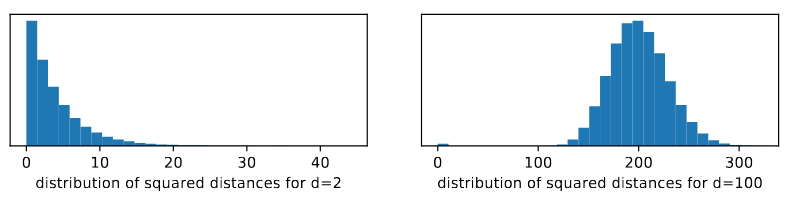
\includegraphics[scale=0.3]{concdist}
	\end{center}
\end{definition}
\newpage
Similarities $p_{ij}$ in the \textbf{input space} are modeled with the \textbf{Gaussian} function
\begin{equation}
	p_{ij} = \frac{1}{Z} \exp\big(- \frac{\lvert\lvert \mathbf{x}_i - \mathbf{x}_j \rvert\rvert^2}{2 \sigma^2}\big)
\end{equation}
with $Z$ being a normalizing term that ensures $\sum_{ij} p_{ij}=1$. The scale $\sigma$ is determined by another parameter called \textbf{perplexity}.

\begin{note}
	In practice, to better represent low connectivity regions, one first computes conditional distributions $p_{i \vdash j}$ and $p_{j \vert i}$ and then sets $p_{ij} \propto p_{i \vert j} + p_{j \vert i}$.
\end{note}
Similarities $q_{ij}$ in the \textbf{embedded} space are modeled with the \textbf{t-Student} function
\begin{equation}
	q_{ij}(\mathbf{y}) = \frac{1}{Z} \cdot \frac{1}{1+ \lvert\lvert \mathbf{y}_i - \mathbf{y}_j \rvert\rvert^2}
\end{equation}
with $Z$ set such that $\sum_{ij}q_{ij}=1$.

\paragraph{Early exaggeration} It's the initial phase of T-SNE where the gradient of the objective
\begin{equation}
	\bigtriangledown D_{KL}(p \vert\vert q(\mathbf{y})) = 4 \cdot \sum_{j}(p_{ij}-q_{ij})\cdot \frac{\mathbf{y}_i - \mathbf{y}_j}{1+\lvert\lvert \mathbf{y}_i - \mathbf{y}_j\rvert\rvert^2}
\end{equation}
is modified by multiplying the values $p_{ij}$ by a factor $\alpha$ in the gradient computations. The optimization loses its probabilistic phase but it helps to escape the local optima and build compact clusters in embedded space representing	 the cluster structure of the input data.

\subsubsection{Comparison}
T-SNE better resolves the local structures of the data and identifies \textbf{clusters}, while MDS better preserves overall distances.
\begin{figure}[!h]
	\hfill
	\subfigure[MDS]{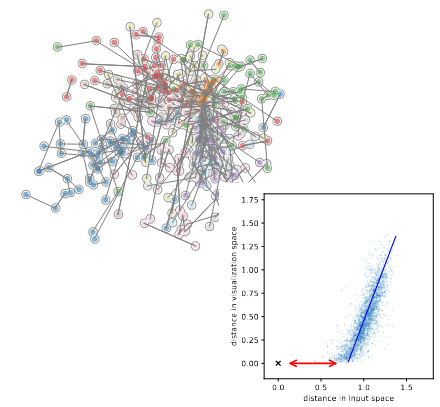
\includegraphics[scale=0.4]{mds2}}
	\hfill
	\subfigure[T-SNE]{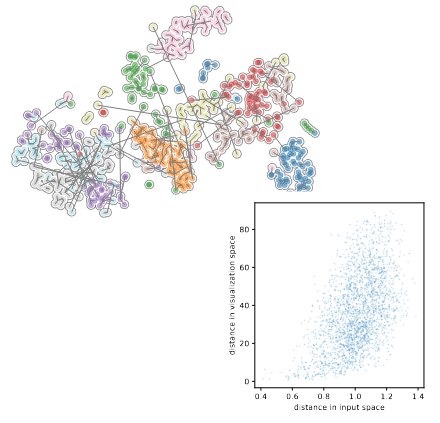
\includegraphics[scale=0.4]{tsne}}
	\hfill
\end{figure}

\subsubsection{Networks}
Usually embedding techniques are used for tabular data but they might also be used for \textbf{network data} (e.g. adjacency matrix). There are different approaches:
\begin{itemize}
	\item Use an embedding techniques that natively works with adjacencies
	\item Consider the adjacency matrix as a data matrix $X \leftarrow A$
	\item Cholesky decomposition $A = LL^T$ and then $X \leftarrow L$
\end{itemize}

\begin{example}
	Embedding of the Game of Thrones relationships.
	\begin{center}
		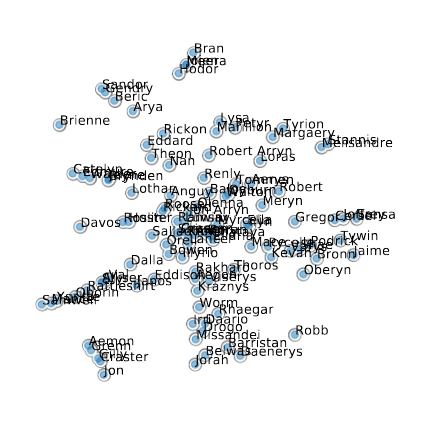
\includegraphics[scale=0.3]{got2}
	\end{center}
\end{example}

\subsubsection{Stringing}
Visualizing the data as an array can be overwhelming when the number of instances and dimensions is large. We can apply \textbf{T-SNE} to the dataset and observe that the embedding coordinates define an \textbf{ordering of instances}. We can the redraw the matrix according to it, getting an easier to interpret visualization.

\begin{figure}[!h]
	\hfill
	\subfigure[Before]{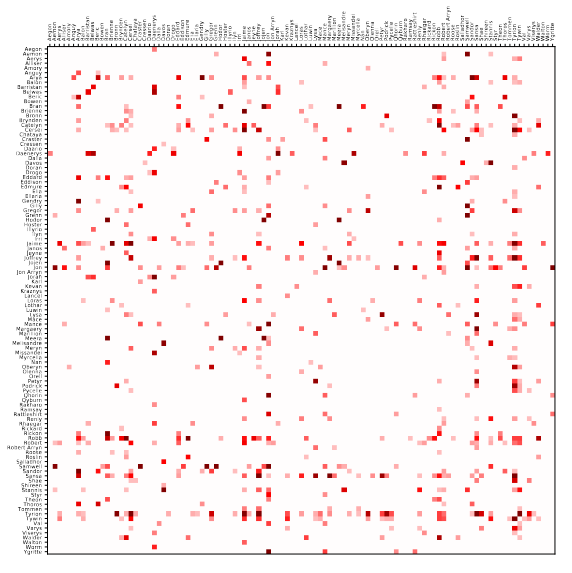
\includegraphics[scale=0.3]{str1}}
	\hfill
	\subfigure[After]{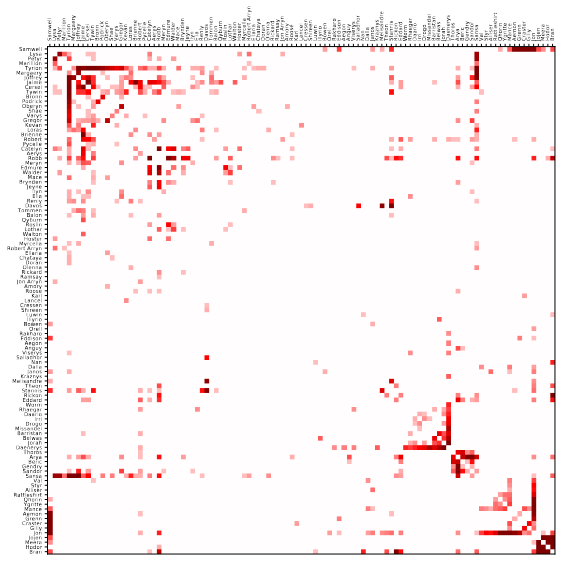
\includegraphics[scale=0.3]{str2}}
	\hfill
\end{figure}

\subsubsection{Limits}
Low-embedding techniques have two main problems:
\begin{itemize}
	\item They could find structures that in reality do not exist
	\item They can distort the geometry of the input data 
\end{itemize}